\chapter{Introducción}
\begin{justify}
    

En Telintec, estamos comprometidos con la mejora continua y la innovación tecnológica. Por ello, hemos desarrollado un sistema integral que centraliza y optimiza los procesos de nuestros departamentos clave: Almacén y Recursos Humanos. Este sistema no solo busca mejorar la eficiencia operativa, sino también establecer una base sólida para una gestión empresarial más ágil y precisa. 
\begin{justify}
Además, estamos implementando herramientas de inteligencia artificial (IA) en nuestra propia operación, con el objetivo de automatizar tareas, generar estadísticas en tiempo real y realizar análisis predictivos que nos permitan anticiparnos a las necesidades de nuestros procesos. La IA nos ayudará a identificar oportunidades de mejora, optimizar recursos y tomar decisiones informadas para el crecimiento sostenido de la empresa. 
\end{justify}
Este manual es una guía para que nuestro equipo adopte el sistema de manera efectiva, entienda sus funcionalidades principales y descubra cómo la tecnología puede convertirse en un aliado estratégico en nuestra operación diaria. Telintec no solo es un sistema, es el futuro de nuestra gestión. 
\end{justify}
\newpage
\pagestyle{fancy}

\section{Objetivo del Manual }
 \begin{justify}
Este manual tiene como objetivo proporcionar a los usuarios una guía detallada para el uso eficiente de la aplicación web Telintec. Incluye instrucciones claras y prácticas para navegar por las distintas funciones y módulos de la plataforma, asegurando que cada usuario pueda aprovechar al máximo las herramientas diseñadas para optimizar las operaciones en los departamentos de Almacén y Recursos Humanos. 
\end{justify}
\section{Descripción y proposito}
\begin{justify}
La aplicación web Telintec es una herramienta integral diseñada para simplificar y automatizar procesos clave en los diferentes departamentos. Su propósito principal es mejorar la gestión de inventarios, solicitudes de material, asistencias y otros procesos administrativos, proporcionando una plataforma intuitiva, eficiente y segura. 
\end{justify}
\section{Usuarios principales}
\begin{itemize}
  \item \textbf{Colaboradores del Departamento de Almacén}\\
  Encargados de la gestión de inventarios, recepción, almacenamiento y distribución de productos. Son los primeros en utilizar el software Telintec de manera activa y principal foco en esta etapa inicial.

  \item \textbf{Responsables de Inventarios}\\
  Se encargan de realizar el seguimiento de existencias, control de stock y organización de los productos dentro del almacén.

  \item \textbf{Personal de Recepción de Productos}\\
  Encargados de registrar la entrada de mercancía, verificar que todo esté en orden y actualizar el sistema con los datos de los productos recibidos.

  \item \textbf{Personal de Despacho y Distribución}\\
  Aseguran la correcta salida de productos del almacén, actualizando el sistema de acuerdo con los pedidos y entregas realizadas.

  \item \textbf{Próximos Usuarios de Otros Departamentos}\\
  A medida que el software se implemente en otros departamentos, como ventas, compras y administración, estos usuarios también comenzarán a interactuar con el sistema para realizar tareas específicas en sus áreas de trabajo.
\end{itemize}



\section{Configuración del sistema}

\begin{itemize}
  \item \textbf{Preferencias del navegador}\\
  Permitir el uso de cookies y almacenamiento local en el navegador. Activar ventanas emergentes para ciertas funcionalidades, como reportes o notificaciones.

  \item \textbf{Requisitos técnicos}\\
  Resolución de pantalla recomendada: 1366x768 o superior para una mejor experiencia visual.\\
  Software complementario (si aplica): Visor de archivos PDF para reportes descargados (Adobe Acrobat Reader o similar). Acceso a herramientas de escaneo si el módulo incluye el uso de hardware externo.

  \item \textbf{Capacitación previa (opcional)}\\
  Conocer las operaciones básicas de la plataforma con el apoyo del manual o videos tutoriales. Familiarización con los procesos internos del departamento correspondiente (Almacén o Recursos Humanos).
\end{itemize}


\section{Inicio de sesión}
\begin{justify}
El inicio de sesión es el primer paso para acceder al sistema Telintec y garantizar que solo los usuarios autorizados puedan utilizar las funciones correspondientes a su departamento, adaptando las funciones disponibles según el rol asignado. Esto asegura que cada empleado tenga acceso únicamente a las herramientas y funciones necesarias para desempeñar sus responsabilidades. Las figuras \ref{fig:session} muestran la interfaz para acceder al sistema. 
\end{justify}


\begin{figure}[ht!]
\centering
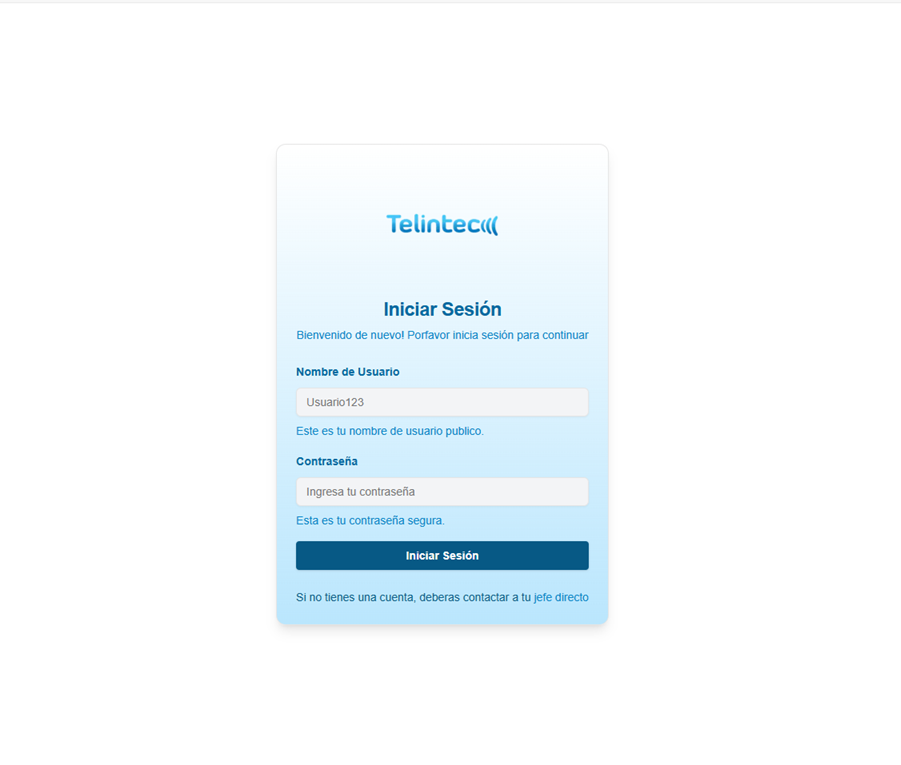
\includegraphics[width=0.6\textwidth]{imgs/inicio de sesion/inicio_sesion_desktop.png}
\caption{Ventana de inicio de sesión.}
\label{fig:login}
\end{figure}

\begin{justify}
A continuación, se describen los pasos para acceder a la plataforma, cómo proceder en caso de olvidar la contraseña y las recomendaciones de seguridad adaptadas a nuestro sistema. 
\end{justify}

\subsection{Acceso según rol de usuario}

\begin{itemize}
    \item  Departamento de Almacén: Los usuarios con este rol tendrán acceso exclusivo a las funcionalidades relacionadas con la gestión de inventarios, movimientos de productos, control de entradas y salidas, y generación de reportes y solicitud de materiales de almacén. 
    \item Departamento de Recursos Humanos: Los usuarios de este rol podrán utilizar las herramientas para la gestión de personal, control de asistencias, evaluación de desempeño, y otras funciones específicas del área de Recursos Humanos. 
\end{itemize}

Ventajas de este Modelo de Acceso:

\begin{itemize}
    \item Seguridad: Protege los datos sensibles asegurando que cada usuario acceda únicamente a la información y funcionalidades relevantes para su departamento. 
    \item Eficiencia: Facilita el uso del sistema al evitar distracciones con herramientas innecesarias para su rol. 
    \item Trazabilidad: Permite rastrear y auditar las acciones realizadas dentro del sistema según el rol del usuario. 
\end{itemize}

\subsection{Proceso de inicio de sesión}
\begin{enumerate}
    \item Ingreso de Credenciales 
    \item Accede a la página de inicio de sesión de Telintec a través de la URL proporcionada por el administrador de la empresa. 
    \item Introduce tu nombre de usuario y contraseña en los campos correspondientes. Estas credenciales serán proporcionadas por el administrador del sistema. 
    \item Haz clic en el botón "Iniciar sesión" para acceder a la plataforma. Si los datos son correctos, serás redirigido al panel principal de tu departamento (Almacén o Recursos Humanos). 
    \item Si no puedes acceder, verifica que tus credenciales sean correctas o consulta el procedimiento en caso de olvido de contraseña. 
\end{enumerate}

\subsection{Recuperación de Contraseña }
\begin{justify}

Actualmente, el sistema Telintec no dispone de una opción automatizada para recuperar contraseñas. En caso de que olvides tu contraseña: 
\end{justify}
\begin{enumerate}
    \item Contacta al equipo de soporte técnico de Telintec a través de los canales establecidos (correo electrónico o línea de soporte). 
    \item Proporciona tus datos de identificación, como nombre completo, correo registrado y departamento, para validar tu identidad. 
    \item El equipo técnico te asistirá en la generación de una nueva contraseña y en la actualización de tus credenciales de acceso. 
    \item Es importante mantener un registro seguro de tus credenciales para evitar interrupciones en el acceso al sistema. 
\end{enumerate}


\subsection{Recomendaciones de seguridad}
\begin{justify}
    Para proteger tu cuenta y los datos manejados por el sistema Telintec, sigue estas recomendaciones: 

\end{justify}

\begin{itemize}
    \item \textbf{Guarda tus credenciales en un lugar seguro:} Mantén un registro de tu usuario y contraseña en un lugar protegido, evitando compartir esta información.
    
    \item \textbf{Cambia tu contraseña regularmente:} Solicita al equipo de soporte que actualice tus credenciales periódicamente para fortalecer la seguridad.
    
    \item \textbf{Evita guardar tu contraseña en dispositivos compartidos:} Si utilizas una computadora o dispositivo no personal, asegúrate de no guardar la contraseña en el navegador.
    
    \item \textbf{Cierra sesión al terminar:} Siempre cierra sesión al finalizar tu uso del sistema, especialmente en dispositivos compartidos.
    
    \item \textbf{Reporta accesos no autorizados y utiliza conexiones seguras:} Si notas alguna actividad inusual o sospechosa en tu cuenta, notifícalo de inmediato al equipo de soporte técnico. Además, accede al sistema solo desde redes confiables para evitar posibles vulnerabilidades.
\end{itemize}

       

